\section{Dataset composition and task groups}
\label{app:data}

The evaluated subset is drawn from the public Cyber Task Horizons release at commit \texttt{178c0da1800f9c07311e1b8d6c61dd8104e7b4ae} (CC BY 4.0). A group is the pair \texttt{benchmark/task\_id}; identical task strings from different benchmarks are distinct groups. The selected agent runs are Claude Sonnet 4.6, Claude Opus 4.6, and GPT-5.5. The selected human traces are expert terminal recordings. Raw logs remain local and are not included in the repository.

\begin{table}[tb]
\centering
\caption{Paired task groups and trace counts in the evaluated subset.}
\label{tab:dataset-counts}
\small
\begin{tabular}{lrrrr}
\toprule
Benchmark & Task groups & Human traces & Agent traces & Random \RecallAtOne \\
\midrule
CyBench & 6 & 8 & 18 & 0.167 \\
InterCode-CTF & 27 & 40 & 81 & 0.037 \\
NYUCTF & 7 & 9 & 21 & 0.143 \\
\midrule
Total / macro & 40 & 57 & 120 & 0.116 \\
\bottomrule
\end{tabular}
\end{table}

\section{Feature construction and evaluation protocol}
\label{app:protocol}

\paragraph{Observed representation.} Human traces contribute recorded terminal command lines. Agent traces contribute command names from \texttt{bash} tool calls. The association baselines use command unigrams, adjacent ordered command bigrams, or adjacent bigrams over coarse action categories. The ProcGrep baseline represents local command patterns using the vendored \href{https://hamidah.me/procgrep/}{ProcGrep} implementation. The command vocabulary, TF--IDF weights, and ProcGrep tokenization are fitted on outer-fold training tasks only. No task prompt, task title, answer, model identifier, output text, timestamp, or file path enters the retrieval features. The 300 Python tool calls in the selected Agent traces are excluded from the primary representation.

\paragraph{Execution-mode head.} A class-balanced logistic-regression model consumes TF--IDF command unigrams and bigrams. For the standalone classification baseline, each task is assigned wholly to one of five outer folds. The negative controls use (i) log command count plus coarse action proportions and (ii) benchmark identity alone. Each control uses the same task folds. The predicted score separates the two dataset trace labels; it is not calibrated as a probability that an unknown real-world operator is an Agent.

\paragraph{Association prototype.} The similarity-only pair ranker combines command-unigram cosine similarity with ordered action-bigram cosine similarity. The mode-aware ranker adds each endpoint's execution-mode score, the score difference, and interaction features. Positives share a benchmark and task ID; negatives use another task within the same benchmark. Training pairs are balanced and task-weighted. In each outer fold, mode scores for training pairs are generated by inner task-grouped out-of-fold prediction; held-out pairs use the model trained without their task. The oracle diagnostic substitutes ground-truth mode labels at inference and is not a deployable system.

\paragraph{Ranking metrics and intervals.} \RecallAtOne is the fraction of queries whose positive task ranks first; ties at the top receive fractional credit. MRR averages the reciprocal rank of the positive task, taking the expectation over a uniform random ordering of exact ties. Query AUC is the probability that a positive task outranks a negative task, with half credit for ties. Metrics are first averaged within each independent task group, then macro-averaged across the three benchmarks. The random \RecallAtOne baseline is the reciprocal of the number of candidate task groups in the query's benchmark. Each 95\% interval uses 5,000 bootstrap replicates: task groups are sampled with replacement within each benchmark, benchmark strata are retained, and the three benchmark means receive equal weight. Paired intervals resample the same task groups for both rankers before taking their difference.

\section{Complete retrieval results}
\label{app:complete-results}

\begin{table}[tb]
\centering
\caption{Human-to-Agent retrieval over all same-benchmark candidate galleries. Values are benchmark-macro estimates; parenthetical ranges are 95\% task-cluster bootstrap intervals.}
\label{tab:retrieval-complete}
\footnotesize
\setlength{\tabcolsep}{3.5pt}
\begin{tabularx}{\linewidth}{>{\raggedright\arraybackslash}Xccc}
\toprule
Method & \RecallAtOne (95\% CI) & MRR (95\% CI) & Query AUC (95\% CI) \\
\midrule
Command unigram cosine & 0.347 [0.165, 0.536] & 0.518 [0.395, 0.638] & 0.740 [0.646, 0.827] \\
Ordered command bigram & 0.265 [0.105, 0.444] & 0.459 [0.346, 0.579] & 0.685 [0.587, 0.780] \\
Ordered action bigram & 0.414 [0.245, 0.576] & 0.561 [0.442, 0.673] & 0.733 [0.637, 0.818] \\
ProcGrep local patterns & 0.287 [0.123, 0.451] & 0.484 [0.372, 0.592] & 0.706 [0.591, 0.802] \\
Prototype: similarity only & 0.346 [0.175, 0.521] & 0.538 [0.429, 0.654] & 0.760 [0.666, 0.839] \\
Prototype: predicted mode & 0.414 [0.231, 0.597] & 0.577 [0.460, 0.697] & 0.775 [0.683, 0.857] \\
Prototype: oracle mode$^{\dagger}$ & 0.346 [0.170, 0.527] & 0.538 [0.420, 0.654] & 0.759 [0.667, 0.840] \\
Random rank & 0.116 & --- & --- \\
\bottomrule
\end{tabularx}
\par\smallskip
\begin{minipage}{\linewidth}\footnotesize
$^{\dagger}$ Ground-truth mode labels are supplied at inference; this diagnostic does not represent a usable detector.
\end{minipage}
\end{table}

\begin{table}[tb]
\centering
\caption{Human-to-Agent \RecallAtOne by benchmark for the four representation baselines.}
\label{tab:benchmark-retrieval}
\small
\begin{tabular}{lrrrrrr}
\toprule
Benchmark & Tasks & Random & Cmd. unigram & Cmd. bigram & Action bigram & ProcGrep \\
\midrule
CyBench & 6 & 0.167 & 0.500 & 0.417 & 0.417 & 0.500 \\
InterCode-CTF & 27 & 0.037 & 0.111 & 0.093 & 0.111 & 0.074 \\
NYUCTF & 7 & 0.143 & 0.429 & 0.286 & 0.714 & 0.286 \\
\bottomrule
\end{tabular}
\end{table}

\begin{figure}[tb]
  \centering
  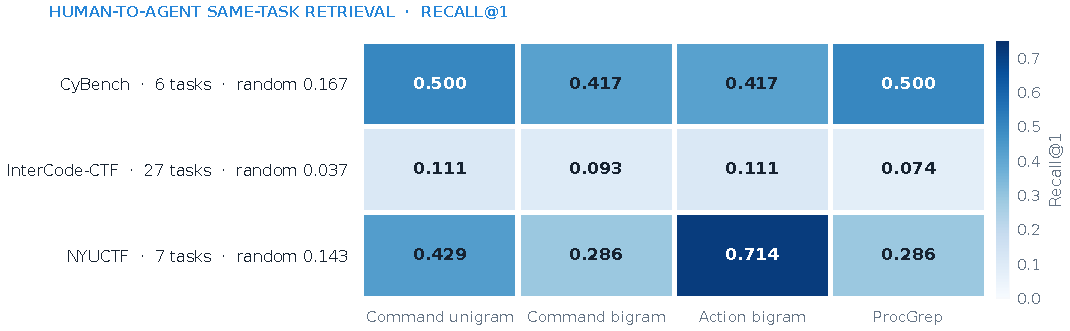
\includegraphics[width=\linewidth]{figureA3_benchmark_retrieval.pdf}
  \caption{Benchmark-level Human-to-Agent task retrieval. Each row gives a benchmark, its number of paired task groups, and its random-ranking baseline. Darker cells indicate higher Recall@1.}
  \label{fig:benchmark-retrieval}
\end{figure}

\section{Mode classification controls and full paired effects}
\label{app:additional-results}

\begin{table}[tb]
\centering
\caption{Task-held-out classification of recorded trace labels. Confusion matrices use rows as true classes (human, Agent) and columns as predicted classes (human, Agent).}
\label{tab:classifier-controls}
\footnotesize
\setlength{\tabcolsep}{3.5pt}
\begin{tabularx}{\linewidth}{>{\raggedright\arraybackslash}Xccc}
\toprule
Features & Balanced accuracy (95\% CI) & Macro-F1 & ROC AUC (95\% CI) \\
\midrule
Command TF--IDF unigrams + bigrams & 0.863 [0.804, 0.915] & 0.854 & 0.945 [0.917, 0.972] \\
Command count + action proportions & 0.650 [0.599, 0.698] & 0.630 & 0.728 [0.674, 0.789] \\
Benchmark identity only & 0.513 [0.488, 0.537] & 0.446 & 0.501 [0.470, 0.534] \\
\bottomrule
\end{tabularx}
\end{table}

The full command n-gram classifier yields the confusion matrix \(\begin{bmatrix}48&9\\14&106\end{bmatrix}\) on the 177 held-out trace records. The command-count/action control yields \(\begin{bmatrix}37&20\\42&78\end{bmatrix}\); the benchmark-only control yields \(\begin{bmatrix}40&17\\81&39\end{bmatrix}\). Task-cluster intervals for balanced accuracy and AUC are shown in Figure~\ref{fig:classifier-controls}.

\begin{figure}[tb]
  \centering
  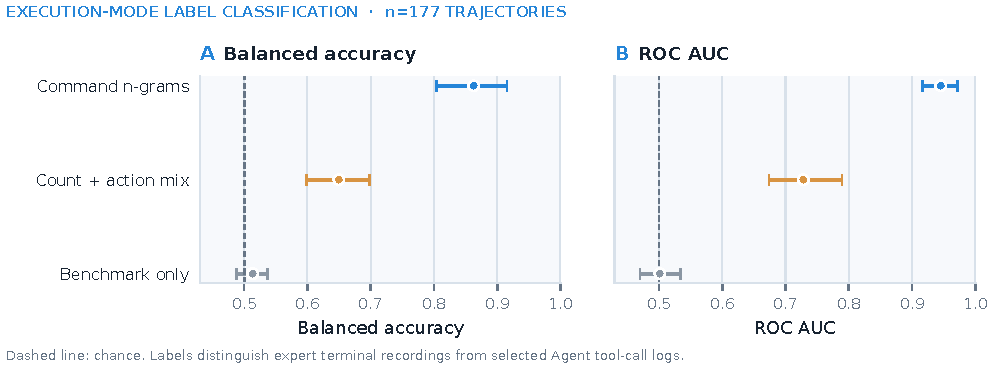
\includegraphics[width=\linewidth]{figureA1_mode_classifier.pdf}
  \caption{Execution-mode label classification and controls. Dashed lines indicate chance-level performance. Because human traces are terminal recordings and Agent traces are tool-call logs, the target labels are confounded with capture modality.}
  \label{fig:classifier-controls}
\end{figure}

\begin{table}[tb]
\centering
\caption{Paired change in ranking metrics from the similarity-only to the mode-aware prototype. Entries are mean differences with 95\% task-cluster bootstrap intervals.}
\label{tab:paired-effects}
\scriptsize
\setlength{\tabcolsep}{2.5pt}
\resizebox{\linewidth}{!}{%
\begin{tabular}{lcccc}
\toprule
Query direction & $n$ & $\Delta$ Recall@1 (95\% CI) & $\Delta$ MRR (95\% CI) & $\Delta$ query AUC (95\% CI) \\
\midrule
Human $\rightarrow$ Agent & 40 & $+0.068\;[-0.012,+0.191]$ & $+0.039\;[-0.006,+0.100]$ & $+0.015\;[-0.005,+0.040]$ \\
Agent $\rightarrow$ Agent (cross-model) & 40 & $+0.012\;[-0.016,+0.051]$ & $+0.008\;[-0.009,+0.030]$ & $+0.011\;[-0.007,+0.033]$ \\
Agent $\rightarrow$ Human & 40 & $+0.024\;[-0.012,+0.068]$ & $+0.021\;[-0.006,+0.055]$ & $+0.014\;[-0.017,+0.044]$ \\
Human $\rightarrow$ Human & 17 & $-0.098\;[-0.189,-0.007]$ & $-0.078\;[-0.139,-0.019]$ & $-0.045\;[-0.079,-0.012]$ \\
\bottomrule
\end{tabular}%
}
\end{table}

\begin{figure}[tb]
  \centering
  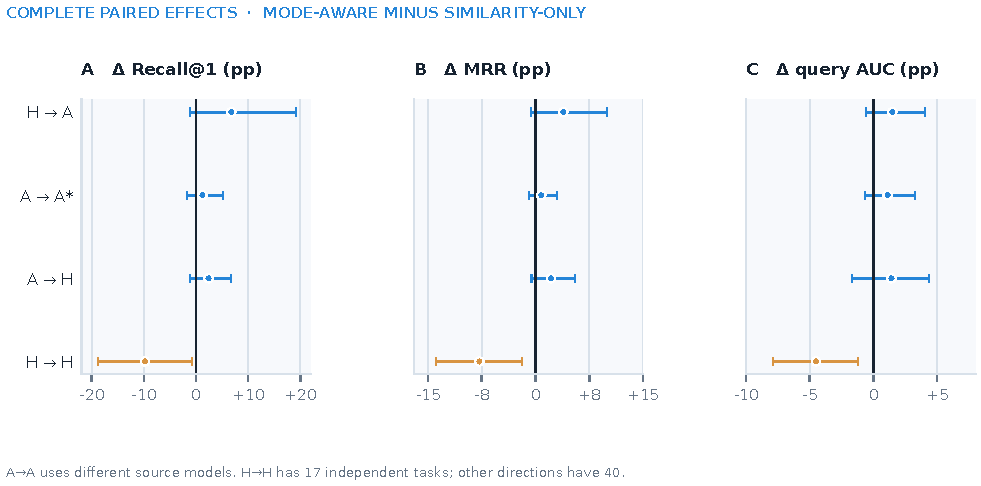
\includegraphics[width=\linewidth]{figureA2_full_directional_effects.pdf}
  \caption{Complete paired effects across Recall@1, MRR, and query AUC. The x-axes are percentage points; points and whiskers are derived from the same task-level paired resamples.}
  \label{fig:full-directional-effects}
\end{figure}

\section{Interpretation scope and next experiment}
\label{app:scope}

The positive retrieval target is a shared CTF task ID. It is not an independently verified shared intrusion, activity, campaign, or organization. The mode-classification labels identify expert terminal records and selected Agent tool-call records, and are therefore inseparable from the logging path in this release. The current evidence supports a reproducible benchmark question about mode-conditioned trace association; it does not estimate real-world APT attribution accuracy.

The next decisive experiment should replay matched red-team activities under four conditions: manual operation, fixed scripts, human-supervised Agent execution, and goal-directed Agent execution. All conditions should use the same host and network telemetry, task snapshots, and logging stack. Independent activity IDs should define same-source positives; distinct activity IDs should define hard negatives. Splits should hold out operators, tasks, and activities together. This design would directly estimate whether mode-aware association reduces false splits and false merges when the behavior logs are collected under equivalent conditions.

\section{Reproduction}
\label{app:reproduction}

From the repository root, install the pinned requirements and run:
\begin{verbatim}
.venv/bin/python scripts/download_public_traces.py
.venv/bin/python scripts/download_crossbenchmark_traces.py
.venv/bin/python scripts/run_crossbenchmark_experiments.py
.venv/bin/python scripts/run_mode_aware_association.py
.venv/bin/python scripts/generate_paper_figures.py
.venv/bin/python -m unittest discover -s tests -v
\end{verbatim}

The figure-generation script reads only the versioned aggregate JSON results and writes vector PDF masters plus 300-dpi PNG previews to \texttt{results/figures/} and \texttt{paper/figures/}. The raw public traces are downloaded locally, verified by the manifest hashes, and excluded from Git. Primary machine-readable outputs are \texttt{results/crossbenchmark\_exploration.json}, \texttt{results/mode\_aware\_association.json}, and the corresponding task-level CSV files.
